% Copyright 2023 Louis Paternault
%
% This work may be distributed and/or modified under the following licences.
%
% LaTeX Project Public Licence
% ----------------------------
%
% This work may be distributed and/or modified under the
% conditions of the LaTeX Project Public License, either version 1.3
% of this license or (at your option) any later version.
% The latest version of this license is in
%   http://www.latex-project.org/lppl.txt
% and version 1.3 or later is part of all distributions of LaTeX
% version 2005/12/01 or later.
%
% Creative Commons by-sa 4.0
% --------------------------
%
% This work may be distributed and/or modified under the
% conditions of the Creative Commons Attribution-ShareAlike 4.0 International
% (CC BY-SA 4.0). The full text of this license is in
% https://creativecommons.org/licenses/by-sa/4.0/

% Compile using LuaLaTeX
%$ lualatex $basename

\documentclass[tikz]{standalone}

\usetikzlibrary{calc}
\usetikzlibrary{angles, arrows.meta, quotes}

\begin{document}

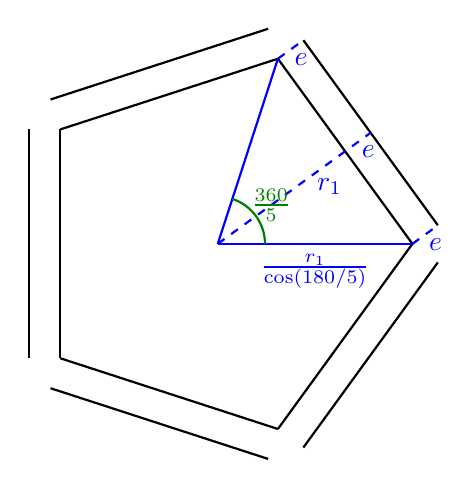
\begin{tikzpicture}[scale=2, thick]%
  \foreach \i in {1, ..., 5} {
    \draw[black]
    ({(\i-1)*360/5}:{1/cos(180/5)})
    --
    ({\i*360/5}:{1/cos(180/5)})
    ;
    \draw[black]
    ($({\i*360/5}:{1/cos(180/5)}) + ({(\i-.5)*360/5}:.2)$)
    --
    ($({(\i-1)*360/5}:{1/cos(180/5)}) + ({(\i-.5)*360/5}:.2)$)
    ;
  }
  \begin{scope}[blue]
    \draw (0, 0) -- (0:{1/cos(180/5)}) node[midway, below]{$\frac{r_1}{\cos(180/5)}$};
    \draw (0, 0) -- ({1*360/5}:{1/cos(180/5)});
    \draw[dashed] (0, 0)
    -- ({.5*360/5}:1) node[near end, below right, inner sep=1pt]{$r_1$}
    -- ({.5*360/5}:1.2) node[midway, below right, inner sep=1pt]{$e$};
    \draw[dashed] (0:{1/cos(180/5)}) -- ++({.5*360/5}:.2) node[midway, below right, inner sep=1pt]{$e$};
    \draw[dashed] ({360/5}:{1/cos(180/5)}) -- ++({.5*360/5}:.2) node[midway, below right, inner sep=1pt]{$e$};
  \end{scope}
  \begin{scope}[green!50!black]
  \coordinate (A) at (0:1);
  \coordinate (B) at (0:0);
  \coordinate (C) at ({360/5}:1);
  \pic[draw, angle radius=6mm, "$\frac{360}{5}$", angle eccentricity=1.4] {angle=A--B--C};
  \end{scope}
\end{tikzpicture}%

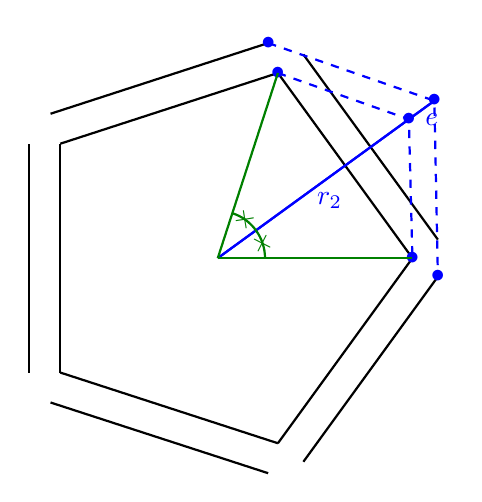
\begin{tikzpicture}[scale=2, thick]%
  \foreach \i in {1, ..., 5} {
    \draw[black]
    ({(\i-1)*360/5}:{1/cos(180/5)})
    --
    ({\i*360/5}:{1/cos(180/5)})
    ;
    \draw[black]
    ($({\i*360/5}:{1/cos(180/5)}) + ({(\i-.5)*360/5}:.2)$)
    --
    ($({(\i-1)*360/5}:{1/cos(180/5)}) + ({(\i-.5)*360/5}:.2)$)
    ;
  }
  \begin{scope}[blue]
    \draw (0, 0)
    -- ({.5*360/5}:1.5) node[midway, below right, inner sep=1pt]{$r_2$}
    node{$\bullet$}
    -- ({.5*360/5}:1.7) node[midway, below right, inner sep=1pt]{$e$}
    node{$\bullet$}
    ;
    \path (0:{1/cos(180/5)}) node{$\bullet$} -- ++({-.5*360/5}:.2) node{$\bullet$};
    \path ({360/5}:{1/cos(180/5)}) node{$\bullet$} -- ++({1.5*360/5}:.2) node{$\bullet$};
    \draw (0, 0) -- ({.5*360/5}:1.7);
    \draw[dashed] ({360/5}:{1/cos(180/5)}) -- ({.5*360/5}:1.5) -- (0:{1/cos(180/5)});
    \draw[dashed] ($({360/5}:{1/cos(180/5)}) + ({1.5*360/5}:.2)$) -- ({.5*360/5}:1.7) -- ($(0:{1/cos(180/5)}) + ({-.5*360/5}:.2)$);
  \end{scope}
  \begin{scope}[green!50!black]
    \draw (0, 0) -- (0:{1/cos(180/5)});
    \draw (0, 0) -- ({360/5}:{1/cos(180/5)});
    \coordinate (A) at (0:0);
    \coordinate (B) at (0:1);
    \coordinate (C) at ({.5*360/5}:1);
    \coordinate (D) at ({360/5}:1);
    \pic[draw, angle radius=6mm] {angle=B--A--C};
    \pic[draw, angle radius=6mm] {angle=C--A--D};
    \draw ({.25*360/5}:3mm) node[rotate={.25*360/5}]{$\times$};
    \draw ({.75*360/5}:3mm) node[rotate={.75*360/5}]{$\times$};
  \end{scope}
\end{tikzpicture}%

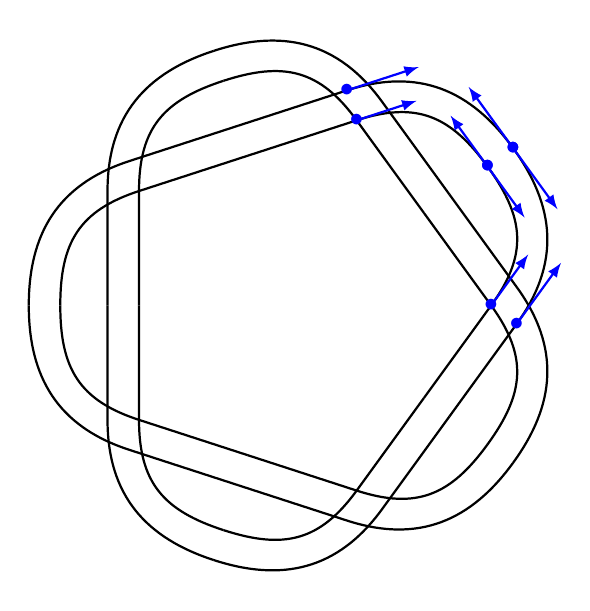
\begin{tikzpicture}[scale=2, thick]%
  \foreach \i in {1, ..., 5} {
    \draw[black]
    ({(\i-.5)*360/5}:1)
    --
    ({\i*360/5}:{1/cos(180/5)})
    ..
    controls
    ($({\i*360/5}:{1/cos(180/5)}) + ({90+360*(\i-.5)/5}:.4)$)
    and
    ($({(\i+1/2)*360/5}:1.5) - ({90+360*(\i+1/2)/5}:.4)$)
    ..
    ({(\i+1/2)*360/5}:1.5)
    ;
    \draw[black]
    ({(\i+1/2)*360/5}:{1.5+.2})
    ..
    controls
    ($({(\i+1/2)*360/5}:{1.5+.2}) - ({90+360*(\i+1/2)/5}:{.4*(1.5+.2)/1.5})$)
    and
    ($({\i*360/5}:{1/cos(180/5)}) + ({(\i-.5)*360/5}:.2) + ({90+360*(\i-.5)/5}:{.4*(1+.2)/1})$)
    ..
    ($({\i*360/5}:{1/cos(180/5)}) + ({(\i-.5)*360/5}:.2)$)
    --
    ({(\i-.5)*360/5}:{1+.2})
    ;
    \draw[black]
    ({(\i-.5)*360/5}:{1})
    --
    ({(\i-1)*360/5}:{1/cos(180/5)})
    ..
    controls
    ($({(\i-1)*360/5}:{1/cos(180/5)}) + ({-90+360*(\i-.5)/5}:.4)$)
    and
    ($({(\i-1-1/2)*360/5}:1.5) - ({-90+360*(\i-1-1/2)/5}:.4)$)
    ..
    ({(\i-1-1/2)*360/5}:1.5)
    ;
    \draw[black]
    ({(\i-.5)*360/5}:{1+.2})
    --
    ($({(\i-1)*360/5}:{1/cos(180/5)}) + ({(\i-.5)*360/5}:.2)$)
    ..
    controls
    ($({(\i-1)*360/5}:{1/cos(180/5)}) + ({(\i-.5)*360/5}:.2) + ({-90+360*(\i-.5)/5}:{.4*(1+.2)/1})$)
    and
    ($({(\i-1-1/2)*360/5}:{1.5+.2}) - ({-90+360*(\i-1-1/2)/5}:{.4*(1.5+.2)/1.5})$)
    ..
    ({(\i-1-1/2)*360/5}:{1.5+.2})
    ;
  }
  \draw[blue, -latex] ({0*360/5}:{1/cos(180/5)}) node{$\bullet$} -- ($({0*360/5}:{1/cos(180/5)}) + ({90+360*(0-.5)/5}:.4)$);
  \draw[blue, -latex] ({1*360/5}:{1/cos(180/5)}) node{$\bullet$} -- ($({1*360/5}:{1/cos(180/5)}) + ({90+360*4/5}:.4)$);
  \draw[blue, -latex] ($({(2-1)*360/5}:{1/cos(180/5)}) + ({(2-.5)*360/5}:.2)$) node{$\bullet$} -- ($({(2-1)*360/5}:{1/cos(180/5)}) + ({(2-.5)*360/5}:.2) + ({-90+360*(2-.5)/5}:{.4*(1+.2)/1})$);
  \draw[blue, -latex] ($({0*360/5}:{1/cos(180/5)}) + ({(0-.5)*360/5}:.2)$) node{$\bullet$} -- ($({0*360/5}:{1/cos(180/5)}) + ({(0-.5)*360/5}:.2) + ({90+360*(0-.5)/5}:{.4*(1+.2)/1})$);
  \draw[blue, -latex] ({(0+1/2)*360/5}:1.5) node{$\bullet$} -- ($({(0+1/2)*360/5}:1.5) - ({90+360*(0+1/2)/5}:.4)$);
  \draw[blue, -latex] ({(0+1/2)*360/5}:1.5) node{$\bullet$} -- ($({(0+1/2)*360/5}:1.5) + ({90+360*(0+1/2)/5}:.4)$);
  \draw[blue, -latex] ({(0+1/2)*360/5}:1.7) node{$\bullet$} -- ($({(0+1/2)*360/5}:1.7) + ({90+360*(0+1/2)/5}:{.4*1.2})$);
  \draw[blue, -latex] ({(0+1/2)*360/5}:1.7) node{$\bullet$} -- ($({(0+1/2)*360/5}:1.7) - ({90+360*(0+1/2)/5}:{.4*1.2})$);
\end{tikzpicture}%

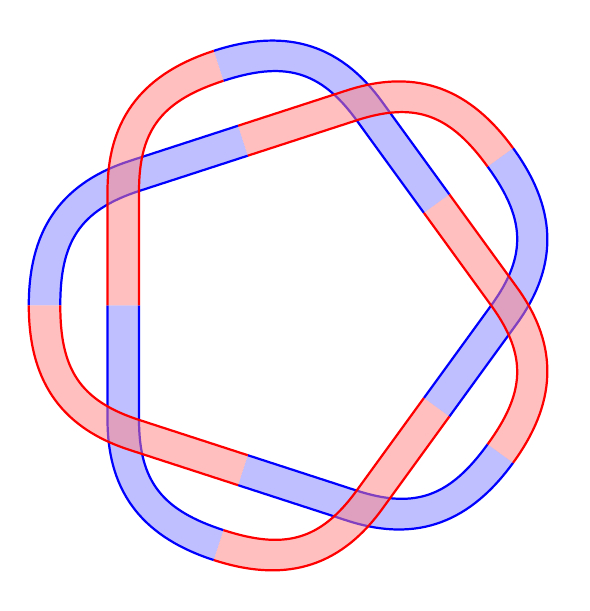
\begin{tikzpicture}[scale=2, thick, fill opacity=.5]%
  \foreach \i in {1, ..., 5} {
    \fill[blue!50!white]
    ({(\i-.5)*360/5}:1)
    --
    ({\i*360/5}:{1/cos(180/5)})
    ..
    controls
    ($({\i*360/5}:{1/cos(180/5)}) + ({90+360*(\i-.5)/5}:.4)$)
    and
    ($({(\i+1/2)*360/5}:1.5) - ({90+360*(\i+1/2)/5}:.4)$)
    ..
    ({(\i+1/2)*360/5}:1.5)
    --
    ({(\i+1/2)*360/5}:{1.5+.2})
    ..
    controls
    ($({(\i+1/2)*360/5}:{1.5+.2}) - ({90+360*(\i+1/2)/5}:{.4*(1.5+.2)/1.5})$)
    and
    ($({\i*360/5}:{1/cos(180/5)}) + ({(\i-.5)*360/5}:.2) + ({90+360*(\i-.5)/5}:{.4*(1+.2)/1})$)
    ..
    ($({\i*360/5}:{1/cos(180/5)}) + ({(\i-.5)*360/5}:.2)$)
    --
    ({(\i-.5)*360/5}:{1+.2})
    ;
    \draw[blue]
    ({(\i-.5)*360/5}:1)
    --
    ({\i*360/5}:{1/cos(180/5)})
    ..
    controls
    ($({\i*360/5}:{1/cos(180/5)}) + ({90+360*(\i-.5)/5}:.4)$)
    and
    ($({(\i+1/2)*360/5}:1.5) - ({90+360*(\i+1/2)/5}:.4)$)
    ..
    ({(\i+1/2)*360/5}:1.5)
    ;
    \draw[blue]
    ({(\i+1/2)*360/5}:{1.5+.2})
    ..
    controls
    ($({(\i+1/2)*360/5}:{1.5+.2}) - ({90+360*(\i+1/2)/5}:{.4*(1.5+.2)/1.5})$)
    and
    ($({\i*360/5}:{1/cos(180/5)}) + ({(\i-.5)*360/5}:.2) + ({90+360*(\i-.5)/5}:{.4*(1+.2)/1})$)
    ..
    ($({\i*360/5}:{1/cos(180/5)}) + ({(\i-.5)*360/5}:.2)$)
    --
    ({(\i-.5)*360/5}:{1+.2})
    ;
  }
  \foreach \i in {1, ..., 5} {
    \fill[red!50!white]
    ({(\i-.5)*360/5}:1)
    --
    ({(\i-1)*360/5}:{1/cos(180/5)})
    ..
    controls
    ($({(\i-1)*360/5}:{1/cos(180/5)}) + ({-90+360*(\i-.5)/5}:.4)$)
    and
    ($({(\i-1-1/2)*360/5}:1.5) - ({-90+360*(\i-1-1/2)/5}:.4)$)
    ..
    ({(\i-1-1/2)*360/5}:1.5)
    --
    ({(\i-1-1/2)*360/5}:{1.5+.2})
    ..
    controls
    ($({(\i-1-1/2)*360/5}:{1.5+.2}) - ({-90+360*(\i-1-1/2)/5}:{.4*(1.5+.2)/1.5})$)
    and
    ($({(\i-1)*360/5}:{1/cos(180/5)}) + ({(\i-.5)*360/5}:.2) + ({-90+360*(\i-.5)/5}:{.4*(1+.2)/1})$)
    ..
    ($({(\i-1)*360/5}:{1/cos(180/5)}) + ({(\i-.5)*360/5}:.2)$)
    --
    ({(\i-.5)*360/5}:{1+.2})
    ;
    \draw[red]
    ({(\i-.5)*360/5}:{1})
    --
    ({(\i-1)*360/5}:{1/cos(180/5)})
    ..
    controls
    ($({(\i-1)*360/5}:{1/cos(180/5)}) + ({-90+360*(\i-.5)/5}:.4)$)
    and
    ($({(\i-1-1/2)*360/5}:1.5) - ({-90+360*(\i-1-1/2)/5}:.4)$)
    ..
    ({(\i-1-1/2)*360/5}:1.5)
    ;
    \draw[red]
    ({(\i-.5)*360/5}:{1+.2})
    --
    ($({(\i-1)*360/5}:{1/cos(180/5)}) + ({(\i-.5)*360/5}:.2)$)
    ..
    controls
    ($({(\i-1)*360/5}:{1/cos(180/5)}) + ({(\i-.5)*360/5}:.2) + ({-90+360*(\i-.5)/5}:{.4*(1+.2)/1})$)
    and
    ($({(\i-1-1/2)*360/5}:{1.5+.2}) - ({-90+360*(\i-1-1/2)/5}:{.4*(1.5+.2)/1.5})$)
    ..
    ({(\i-1-1/2)*360/5}:{1.5+.2})
    ;
  }
\end{tikzpicture}%
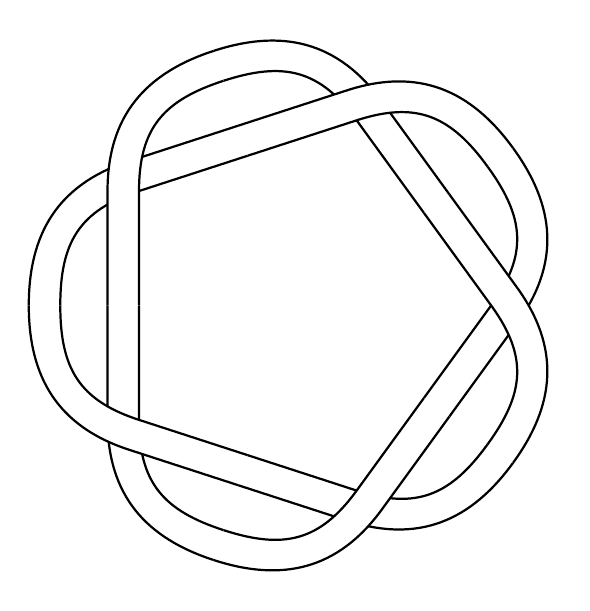
\begin{tikzpicture}[scale=2, thick]%
  \foreach \i in {1, ..., 5} {
    \fill[white]
    ({(\i-.5)*360/5}:1)
    --
    ({\i*360/5}:{1/cos(180/5)})
    ..
    controls
    ($({\i*360/5}:{1/cos(180/5)}) + ({90+360*(\i-.5)/5}:.4)$)
    and
    ($({(\i+1/2)*360/5}:1.5) - ({90+360*(\i+1/2)/5}:.4)$)
    ..
    ({(\i+1/2)*360/5}:1.5)
    --
    ({(\i+1/2)*360/5}:{1.5+.2})
    ..
    controls
    ($({(\i+1/2)*360/5}:{1.5+.2}) - ({90+360*(\i+1/2)/5}:{.4*(1.5+.2)/1.5})$)
    and
    ($({\i*360/5}:{1/cos(180/5)}) + ({(\i-.5)*360/5}:.2) + ({90+360*(\i-.5)/5}:{.4*(1+.2)/1})$)
    ..
    ($({\i*360/5}:{1/cos(180/5)}) + ({(\i-.5)*360/5}:.2)$)
    --
    ({(\i-.5)*360/5}:{1+.2})
    ;
    \draw[black]
    ({(\i-.5)*360/5}:1)
    --
    ({\i*360/5}:{1/cos(180/5)})
    ..
    controls
    ($({\i*360/5}:{1/cos(180/5)}) + ({90+360*(\i-.5)/5}:.4)$)
    and
    ($({(\i+1/2)*360/5}:1.5) - ({90+360*(\i+1/2)/5}:.4)$)
    ..
    ({(\i+1/2)*360/5}:1.5)
    ;
    \draw[black]
    ({(\i+1/2)*360/5}:{1.5+.2})
    ..
    controls
    ($({(\i+1/2)*360/5}:{1.5+.2}) - ({90+360*(\i+1/2)/5}:{.4*(1.5+.2)/1.5})$)
    and
    ($({\i*360/5}:{1/cos(180/5)}) + ({(\i-.5)*360/5}:.2) + ({90+360*(\i-.5)/5}:{.4*(1+.2)/1})$)
    ..
    ($({\i*360/5}:{1/cos(180/5)}) + ({(\i-.5)*360/5}:.2)$)
    --
    ({(\i-.5)*360/5}:{1+.2})
    ;
  }
  \foreach \i in {1, ..., 5} {
    \fill[white]
    ({(\i-.5)*360/5}:1)
    --
    ({(\i-1)*360/5}:{1/cos(180/5)})
    ..
    controls
    ($({(\i-1)*360/5}:{1/cos(180/5)}) + ({-90+360*(\i-.5)/5}:.4)$)
    and
    ($({(\i-1-1/2)*360/5}:1.5) - ({-90+360*(\i-1-1/2)/5}:.4)$)
    ..
    ({(\i-1-1/2)*360/5}:1.5)
    --
    ({(\i-1-1/2)*360/5}:{1.5+.2})
    ..
    controls
    ($({(\i-1-1/2)*360/5}:{1.5+.2}) - ({-90+360*(\i-1-1/2)/5}:{.4*(1.5+.2)/1.5})$)
    and
    ($({(\i-1)*360/5}:{1/cos(180/5)}) + ({(\i-.5)*360/5}:.2) + ({-90+360*(\i-.5)/5}:{.4*(1+.2)/1})$)
    ..
    ($({(\i-1)*360/5}:{1/cos(180/5)}) + ({(\i-.5)*360/5}:.2)$)
    --
    ({(\i-.5)*360/5}:{1+.2})
    ;
    \draw[black]
    ({(\i-.5)*360/5}:{1})
    --
    ({(\i-1)*360/5}:{1/cos(180/5)})
    ..
    controls
    ($({(\i-1)*360/5}:{1/cos(180/5)}) + ({-90+360*(\i-.5)/5}:.4)$)
    and
    ($({(\i-1-1/2)*360/5}:1.5) - ({-90+360*(\i-1-1/2)/5}:.4)$)
    ..
    ({(\i-1-1/2)*360/5}:1.5)
    ;
    \draw[black]
    ({(\i-.5)*360/5}:{1+.2})
    --
    ($({(\i-1)*360/5}:{1/cos(180/5)}) + ({(\i-.5)*360/5}:.2)$)
    ..
    controls
    ($({(\i-1)*360/5}:{1/cos(180/5)}) + ({(\i-.5)*360/5}:.2) + ({-90+360*(\i-.5)/5}:{.4*(1+.2)/1})$)
    and
    ($({(\i-1-1/2)*360/5}:{1.5+.2}) - ({-90+360*(\i-1-1/2)/5}:{.4*(1.5+.2)/1.5})$)
    ..
    ({(\i-1-1/2)*360/5}:{1.5+.2})
    ;
  }
\end{tikzpicture}%
\end{document}
